\section{Experiments}
\label{sec:experiments}

The experiments follow three questions. Does early state transfer carry
skill-relevant information? Does that transfer weaken before dependence
on the skill does? Can source-cache replacement restore part of the late
transfer deficit?

\subsection{Experimental setup}
\label{sec:setup}
\label{sec:cells}

\paragraph{Tasks and models.}
We pair MedCalc-Bench \citep{khandekar2024medcalc} with skills from
SRA-Bench, a benchmark that pairs questions with reusable skill documents
\citep{su2026srabench}, covering $1{,}100$ questions from $55$
clinical calculators. We also use SRA-Bench's TheoremQA subset, with $747$
questions and $320$ skills. TheoremQA tests the application of theorems
across mathematics, physics, electrical engineering and computer science,
and finance \citep{chen2023theoremqa}, extending the evaluation beyond
clinical calculations. Each question receives its designated skill.
Skill selection is held fixed.

The four main models are Qwen3-8B \citep{yang2025qwen3},
Mistral-7B-Instruct-v0.3 \citep{jiang2023mistral}, Llama-3.1-8B-Instruct
\citep{grattafiori2024llama3} and DeepSeek-LLM-7B-Chat
\citep{deepseek2024llm}. The depth study covers all eight combinations of
model and benchmark (Table~\ref{tab:paireddepth}). Qwen3-8B and Mistral on
TheoremQA use regenerated answers with independently checked grading
(Appendix~\ref{app:limits}).
Models generate step-by-step answers without tools using greedy decoding,
and the benchmark scorers evaluate those answers. On the full MedCalc benchmark, Qwen3-8B
achieves $74.2\%$ accuracy with the correct skill, $34.5\%$ without one,
and $31.5\%$ with an unrelated skill.

% Queue the control table before the depth figures.
\begin{table*}[t]
\centering
\caption{Early transfer at $L2$ and fixed-layer controls at $L8$.
Entries are accuracy (\%), with separate question/skill counts ($n/G$)
for each block. $L2$ establishes effective early transfer across all eight
combinations. $L8$ tests content and position controls at a fixed depth,
which is already beyond some transfer boundaries. Sample selection is
specified in Section~\ref{sec:setup}.}
\label{tab:probe}
\normalfont\rmfamily\fontsize{9}{11}\selectfont
\renewcommand{\arraystretch}{1.18}
\setlength{\tabcolsep}{2pt}
\arrayrulecolor{TableInk}
\setlength{\heavyrulewidth}{0.7pt}
\setlength{\lightrulewidth}{0.3pt}
\setlength{\aboverulesep}{2pt}
\setlength{\belowrulesep}{2.5pt}
\begin{tabularx}{\textwidth}{@{}l*{8}{>{\centering\arraybackslash}X}@{}}
\toprule
\rowcolor[HTML]{E4F4FA}
Intervention & \multicolumn{2}{c}{\textbf{Qwen3-8B}} & \multicolumn{2}{c}{\textbf{Mistral-7B}} & \multicolumn{2}{c}{\textbf{Llama-3.1-8B}} & \multicolumn{2}{c}{\textbf{DeepSeek-7B}} \\
\cmidrule(lr){2-3}\cmidrule(lr){4-5}\cmidrule(lr){6-7}\cmidrule(l){8-9}
 & MedCalc & TheoremQA & MedCalc & TheoremQA & MedCalc & TheoremQA & MedCalc & TheoremQA \\
\midrule
\multicolumn{9}{l}{\textit{Early validation at $L2$}} \\
$n/G$ & $97/11$ & $61/51$ & $35/13$ & $61/51$ & $112/20$ & $92/71$ & $25/13$ & $54/45$ \\
\rowcolor[HTML]{E4F4FA}
\textbf{Correct skill span} & \textbf{89.7} & \textbf{93.4} & \textbf{68.6} & \textbf{85.2} & \textbf{90.2} & \textbf{76.1} & \textbf{56.0} & \textbf{57.4} \\
Correct span, permuted & 2.1 & 14.8 & 5.7 & 11.5 & 6.2 & 8.7 & 12.0 & 1.9 \\
Norm-matched noise & 4.1 & 14.8 & 5.7 & 6.6 & 1.8 & 6.5 & 4.0 & 1.9 \\
\midrule
\multicolumn{9}{l}{\textit{Fixed-layer controls at $L8$}} \\
$n/G$ & $135/14$ & $57/49$ & $35/13$ & $61/51$ & $112/20$ & $92/71$ & $25/13$ & $54/45$ \\
Correct skill donor & 91.9 & 100.0 & 100.0 & 100.0 & 100.0 & 100.0 & 100.0 & 100.0 \\
Wrong skill receiver & 0.0 & 0.0 & 0.0 & 0.0 & 0.0 & 0.0 & 0.0 & 0.0 \\
Correct skill span & 81.5 & 78.9 & 20.0 & 37.7 & 33.0 & 23.9 & 8.0 & 11.1 \\
Last prompt token & 3.0 & 10.5 & 5.7 & 1.6 & 2.7 & 12.0 & 0.0 & 1.9 \\
Last 16 prompt tokens & 5.9 & 12.3 & 8.6 & 6.6 & 2.7 & 4.3 & 4.0 & 11.1 \\
\addlinespace[2pt]
Correct matched prefix & 59.3 & 71.9 & 17.1 & 37.7 & 35.7 & 22.8 & 12.0 & 7.4 \\
Other-skill matched prefix & 4.4 & 14.0 & 2.9 & 8.2 & 8.0 & 9.8 & 8.0 & 5.6 \\
\addlinespace[2pt]
Correct span, permuted & 4.4 & 22.8 & 14.3 & 14.8 & 4.5 & 14.1 & 4.0 & 5.6 \\
Norm-matched noise & 2.2 & 19.3 & 8.6 & 4.9 & 4.5 & 9.8 & 4.0 & 0.0 \\
Identity patch & 0.0 & 0.0 & 0.0 & 0.0 & 0.0 & 0.0 & 0.0 & 0.0 \\
\bottomrule
\end{tabularx}

\end{table*}

\paragraph{Analysis populations.}
We select questions using earlier with-skill and without-skill outcomes,
then re-evaluate unmodified runs, or baselines, under each protocol.
For skill-level screening, we retain a skill only if the wrong-skill
receiver answers none of its sampled questions correctly.

For Qwen3-8B/MedCalc, we use $97$ questions for $L2$ validation
and $135$ for $L8$ controls
(Table~\ref{tab:probe}), $134$ for common depth curves
(Figure~\ref{fig:transferreading}), $124$ for the paired-outcome check
(\S\ref{sec:depth}), and $114$ for repair and path cuts
(Figure~\ref{fig:mechanism}). The control donor answers $124/135$
correctly. The common depth set intersects transfer eligibility with
correct-with-skill, incorrect-without-skill knockout outcomes.
The paired check also requires correct donor answers under both protocols.

All $L2$ cells and the added $L8$ cells also require correct donor and
incorrect no-skill baselines. Each block reports its own $n/G$, since
their eligible sets can differ. Repair uses that rule plus an incorrect receiver for each
item. Llama and DeepSeek reuse fixed candidate pools selected by earlier
models. Intervention estimates are conditional on these selection rules.
Each depth panel uses common question IDs for its two interventions.
Repair and path tests likewise share question IDs within each model and
task combination, using their own fresh-baseline screen.
Appendix~\ref{app:setup} details the distinct selection rules.


The complete-source study uses separate fixed historical pools totaling
$580$ model and question pairs and retains fresh baseline failures.
It compares an unrelated-skill receiver (Wrong) with a fixed unrelated
text matched to the source length (Neutral). All complete-source conditions use matched attention and decoding settings.
Appendix~\ref{app:state-completeness} gives the pools and protocol.

\paragraph{Protocol consistency.}
Historical Qwen3-8B and regenerated Qwen/Mistral TheoremQA runs use
 different attention implementations for transfer and knockout.
Llama and DeepSeek use matching implementations. Repair and path cuts share a protocol
with fresh baselines. Identity controls copy receiver states back to
their original positions and reproduce its output tokens exactly.
Resetting the TheoremQA evaluator before every answer
and reversing grading order preserve the labels. Implementation details
and corrections are in Appendix~\ref{app:setup}.

\subsection{Validation of skill-state transfer}
\label{sec:battery}

\paragraph{Early transfer recovery.}
At layer $2$, correct-skill states give $56.0\%$ to $93.4\%$ accuracy
across all eight combinations, compared with $1.9\%$ to $14.8\%$ for
permuted states and $1.8\%$ to $14.8\%$ for norm-matched noise
(Table~\ref{tab:probe}, upper block). Donors are correct and receivers
incorrect on these screened sets, so the accuracies also give the
percentage of donor gain recovered. This establishes effective early
transfer before comparing its depth profile with skill dependence.

% Queue the paired depth displays together.
\begin{figure*}[t]
\centering
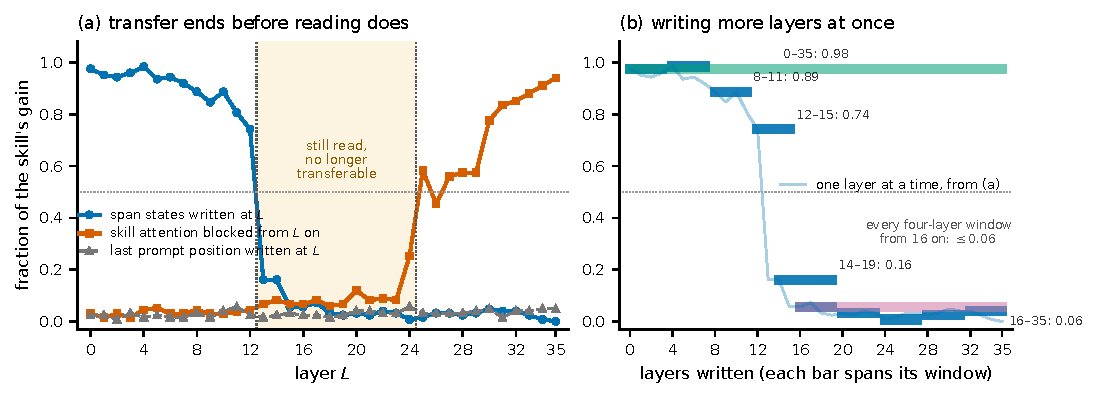
\includegraphics[width=\textwidth]{fig-transfer-reading.pdf}
\caption{State transfer weakens before source-attention dependence across
eight combinations of model and task. Rows show MedCalc (top) and TheoremQA
(bottom), with models aligned by column. Mint: recovery $\rho(L)$ in the wrong-skill
receiver. Pink dash-dotted: dependence $d(L)$ in the original correct-skill
run. Each panel uses common eligible questions with each protocol's own
baselines. $G$ counts skills. The horizontal line marks $0.5$ and mint/pink vertical markers locate
the first boundaries $T/R$. Shading spans their interval
(Table~\ref{tab:paireddepth}). Later threshold crossings remain visible. Knockout
blocks both skill reading and within-skill attention. Every layer is measured.}
\Description{Eight compact line plots in two rows and four columns show mint transfer-recovery curves and pink dash-dotted source-dependence curves on common eligible populations. The top row is MedCalc and the bottom row TheoremQA. Columns are Qwen3-8B, Mistral-7B, Llama-3.1-8B and DeepSeek-7B. Light bands mark intervals between first half-effect boundaries.}
\label{fig:transferreading}
\end{figure*}



\paragraph{Content and position controls at a fixed depth.}
The lower block of Table~\ref{tab:probe} retains the $L8$ controls.
For Qwen3-8B/MedCalc, skill-span transfer answers $110/135$ questions
correctly, against the donor's $124/135$ and receiver's zero, recovering
$0.89$ of the donor's gain. Last-token and last-$16$-token writes have
smaller effects but also replace fewer positions. The matched-prefix
comparison copies equal numbers of leading skill positions and recovers
$0.65$ with correct content versus $0.05$ with unrelated content.
Permuting positions or injecting norm-matched noise gives little recovery.
This noise preserves the Euclidean length of the skill-state change.
Rescaling the correct patch to the receiver's norm still recovers $0.87$.
These controls support a role for the skill's content and arrangement.
At $L8$, several other models have already crossed their transfer boundary
(Figure~\ref{fig:transferreading}).

\paragraph{Cross-question transfer.}
\label{sec:whose}
In the main prompt order, the skill precedes the question. Causal attention
prevents those skill states from encoding a later question. We additionally
place the skill after the question and take donor states from other
questions using the same skill. For Qwen3-8B/MedCalc, these states recover
$0.98$ at layer $8$ on $151$ eligible items from $17$ calculators, close to $1.02$ for
a donor answering the current question. At layer $16$, the values separate
to $0.29$ and $0.49$. Early transfer thus carries information shared across
questions, with greater question sensitivity later.

% Queue the repair display for the page following the depth comparison.
\begin{figure*}[t]
\centering
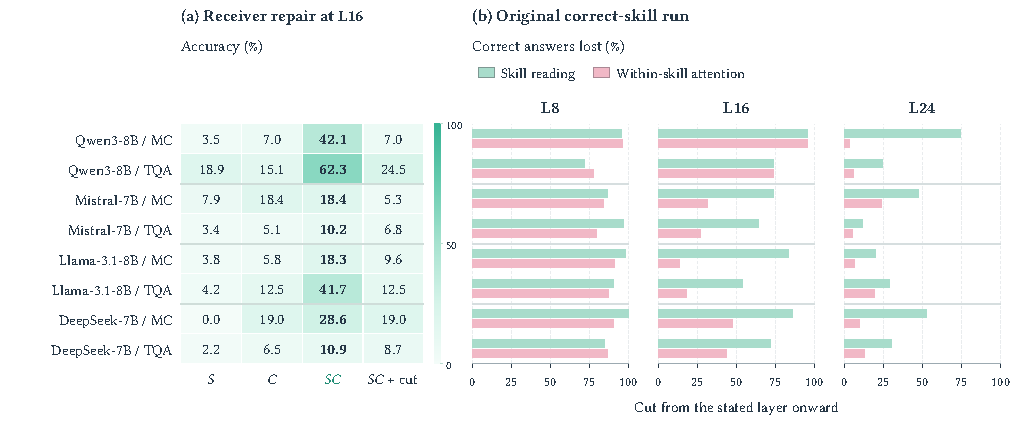
\includegraphics[width=\textwidth]{fig-mechanism-results.pdf}
\caption{Repair and attention cuts across four models and two benchmarks.
MC denotes MedCalc and TQA denotes TheoremQA.
(a) Receiver accuracy at $L16$ for state replacement ($S$), cache
replacement ($C$), joint repair ($SC$), and joint repair with a reading
cut from $L17$ onward ($SC+\mathrm{cut}$).
(b) Correct answers lost in the original correct-skill run under cuts
from $L8$, $L16$ or $L24$ onward during prefill and decoding.
Skill reading blocks reader-to-source attention. Within-skill attention
blocks source-to-source attention. Each row uses the same
questions in both panels, with counts in Table~\ref{tab:mechanism-contrasts}.
Higher values mean better recovery in (a)
and greater disruption in (b). Layer numbers index each model's blocks.}
\Description{Eight shared rows pair each of four models with MedCalc and TheoremQA. The left mint heatmap gives all 32 repair accuracies at layer 16 on a fixed zero-to-100-percent scale, with the joint-repair column bold. Three aligned panels on the right show 48 horizontal bars at layers 8, 16 and 24. Mint bars denote Skill reading cuts and pink bars denote Within-skill attention cuts. All three horizontal axes run from zero to 100 percent of originally correct answers lost. At layer 24, reading cuts cause larger losses than within-skill cuts in all eight rows, with varying magnitudes.}
\label{fig:mechanism}
\end{figure*}

\begin{samepage}
\subsection{Weak transfer with persistent source dependence}
\label{sec:where}
\label{sec:depth}
\label{sec:ladder}

\paragraph{Depth separation.}
Early transfer is effective, but it weakens before source dependence does.
Figure~\ref{fig:transferreading} shows the full curves, and
Table~\ref{tab:paireddepth} summarizes their boundaries.
\end{samepage}

The dependence boundary follows the transfer boundary in all eight
comparisons. The gaps are $8$ to $20$ layers, or $22.2\%$ to $62.5\%$ of
model depth (Table~\ref{tab:paireddepth}). 
\begin{table*}[t]
\centering
\caption{Main depth comparison across four open-weight models and two benchmarks.
$n/G$ gives common eligible questions/skill groups. $T$ and $R$ are the first
half-effect crossings for transfer ($\rho<0.5$) and aggregate source dependence
($d\le0.5$). $\Delta=R-T$ is in layers. $\Delta/D$ normalizes the gap
by the model's layer count. All eight cells use audited common-item populations.}
\label{tab:paireddepth}
\normalfont\rmfamily\fontsize{9}{11}\selectfont
\renewcommand{\arraystretch}{1.18}
\setlength{\tabcolsep}{3pt}
\begin{tabular*}{\textwidth}{@{\extracolsep{\fill}}lrrrrrrrrrr@{}}
\toprule
Model & \multicolumn{5}{c}{MedCalc-Bench} & \multicolumn{5}{c}{TheoremQA} \\
\cmidrule(lr){2-6}\cmidrule(l){7-11}
 & $n/G$ & $T$ & $R$ & $\Delta$ & $\Delta/D$ (\%) & $n/G$ & $T$ & $R$ & $\Delta$ & $\Delta/D$ (\%) \\
\midrule
Qwen3-8B & $134/14$ & $13$ & $25$ & \textbf{12} & \textbf{33.3} & $82/66$ & $13$ & $21$ & \textbf{8} & \textbf{22.2} \\
Mistral-7B & $46/16$ & $7$ & $27$ & \textbf{20} & \textbf{62.5} & $72/58$ & $7$ & $19$ & \textbf{12} & \textbf{37.5} \\
Llama-3.1-8B & $112/20$ & $7$ & $18$ & \textbf{11} & \textbf{34.4} & $92/71$ & $6$ & $18$ & \textbf{12} & \textbf{37.5} \\
DeepSeek-7B & $25/13$ & $6$ & $21$ & \textbf{15} & \textbf{50.0} & $54/45$ & $4$ & $19$ & \textbf{15} & \textbf{50.0} \\
\bottomrule
\end{tabular*}

\end{table*}

\paragraph{A representative depth profile.}
For Qwen3-8B/MedCalc, recovery drops from $0.73$
at layer $12$ to $0.16$ at $13$ and stays below $0.08$ from $15$ onward.
Dependence remains $0.93$ at $13$ and $0.75$ at $24$.
Throughout layers $13$ to $24$, transfer restores less than half of the
donor's gain while knockout removes more than half of the originally
correct answers (Figure~\ref{fig:transferreading}).

\paragraph{Paired outcomes and robustness.}
The paired check confirms the separation on individual questions. For
Qwen3-8B/MedCalc, both interventions yield incorrect answers on $100/124$
($80.6\%$) questions at layer $13$, and $113/124$ ($91.1\%$) at $16$ (Appendix~\ref{app:joint-failure}). The boundary ordering also
holds at thresholds $0.4$ and $0.6$ in all eight comparisons. Broader
screening and later threshold crossings appear in Appendix~\ref{app:fullscale}.

\subsection{Partial restoration with source-cache replacement}
\label{sec:mechanism}

\paragraph{Testing an omitted source component.}
Figure~\ref{fig:mechanism} compares all eight model and task combinations,
separating receiver repair at $L16$ (panel a) from attention cuts in the
original correct-skill run at $L8$, $L16$ and $L24$ (panel b).

\paragraph{Repair gains in the receiver.}
Adding caches improves accuracy over state transfer alone in all eight
layer-$16$ comparisons, by $6.8$ to $43.4$ percentage points
(Figure~\ref{fig:mechanism}a). Joint-repair accuracy ranges from $10.2\%$
to $62.3\%$. For Qwen3-8B/MedCalc, $S$, $C$ and $SC$ answer $4$, $8$
and $48$ of $114$ questions correctly ($3.5\%$, $7.0\%$, $42.1\%$).
The cache benefit is $\Delta_{\mathrm{cache}}=(48-4)/114$, or $38.6$
percentage points. The accuracy interaction is
$\Gamma=(48-4-8+0)/114$, or $31.6$ points (Eq.~\eqref{eq:repair-effects}).
At layer $24$, $SC$ reaches $25.4\%$, versus $0.9\%$ for $S$ and
$18.4\%$ for $C$. The added benefit of states alongside caches varies.
For Mistral/MedCalc at $L16$, $SC$ and $C$ both reach $18.4\%$, with
$\Gamma=-7.9$ points. Table~\ref{tab:mechanism-contrasts} reports all
individual conditions and contrasts.

\paragraph{Reading under joint repair.}
Reading cuts reduce joint-repair accuracy by $2.2$ to $37.7$ points
across all eight layer-$16$ comparisons. For Qwen3-8B/MedCalc, accuracy falls
from $42.1\%$ to $7.0\%$, giving $\Delta_{\mathrm{read}}=(48-8)/114$,
or $35.1$ points. Thus the cross-model improvement from adding caches
coexists with continued use of the skill. The Qwen3-8B/MedCalc result at
$L24$ differs: the cut gives $27.2\%$ versus $25.4\%$ without it.
Appendix~\ref{app:mechanism} documents the layer grid and checks sensitivity
to outputs stopped at the generation limit.

\paragraph{Attention paths in the original run.}
Figure~\ref{fig:mechanism}(b) tests the original correct-skill execution.
At $L8$, both types of cut cause large losses across the eight rows.
At $L24$, Skill reading loses $11.9\%$ to $74.6\%$ of correct answers,
exceeding Within-skill attention by $6.8$ to $71.1$ points in every row.
The Qwen3-8B/MedCalc contrast is $74.6\%$ versus $3.5\%$.
At this measured depth, later positions' access to the skill has a
larger effect than attention among skill positions across all eight settings.

% Let the complete-source table follow the repair figure on the next page.
\begin{table*}[t]
\centering
\caption{Recovery with complete source KV and receiving-history controls.
Entries are accuracy (\%). $C_{\mathrm{all}}$ copies all source KV,
$SC@L$ adds a state write at layer $L$, and $B$ copies only other prefix KV.
Full copies the complete prefix and equals the donor. Replay copies all
source KV and recomputes the later prompt. Wrong and Neutral are defined
in Section~\ref{sec:setup}, with separate sample counts in Table~\ref{tab:state-baselines}.}
\label{tab:state-completeness}
\normalfont\rmfamily\fontsize{9}{11}\selectfont
\renewcommand{\arraystretch}{1.18}
\setlength{\tabcolsep}{2.5pt}
% Keep the local rules black, including the shared tabular hook.
\colorlet{TableInk}{black}
\arrayrulecolor{black}
\setlength{\heavyrulewidth}{0.7pt}
\setlength{\lightrulewidth}{0.3pt}
\setlength{\aboverulesep}{2pt}
\setlength{\belowrulesep}{2.5pt}
\begin{tabularx}{\textwidth}{@{}lc*{8}{>{\centering\arraybackslash}X}@{}}
\toprule
Model / task & Context & Base & $C_{\mathrm{all}}$ & $SC@8$ & $SC@16$ & $SC@24$ & $B$ & \shortstack{Full\\(= donor)} & Replay \\
\midrule
Qwen3-8B / MC & Wrong & 4.8 & 29.8 & 91.9 & 41.9 & 25.8 & 2.4 & 97.6 & 96.8 \\
 & Neutral & 4.0 & 25.0 & 91.1 & 28.2 & 26.6 & 8.1 & 97.6 & 96.8 \\
\addlinespace[2pt]
Qwen3-8B / TQA & Wrong & 6.3 & 58.7 & 95.2 & 60.3 & 50.8 & 20.6 & 96.8 & 98.4 \\
 & Neutral & 25.4 & 73.0 & 84.1 & 65.1 & 71.4 & 34.9 & 96.8 & 98.4 \\
\addlinespace[2pt]
Mistral-7B / MC & Wrong & 6.5 & 15.2 & 56.5 & 15.2 & 13.0 & 4.3 & 91.3 & 89.1 \\
 & Neutral & 6.5 & 17.4 & 39.1 & 17.4 & 17.4 & 19.6 & 91.3 & 89.1 \\
\addlinespace[2pt]
Mistral-7B / TQA & Wrong & 3.1 & 10.8 & 49.2 & 9.2 & 13.8 & 24.6 & 93.8 & 93.8 \\
 & Neutral & 4.6 & 23.1 & 43.1 & 21.5 & 21.5 & 27.7 & 93.8 & 93.8 \\
\addlinespace[2pt]
Llama-3.1-8B / MC & Wrong & 1.8 & 16.1 & 73.2 & 17.0 & 16.1 & 1.8 & 96.4 & 96.4 \\
 & Neutral & 8.0 & 27.7 & 48.2 & 25.9 & 25.9 & 4.5 & 96.4 & 96.4 \\
\addlinespace[2pt]
Llama-3.1-8B / TQA & Wrong & 5.4 & 43.5 & 45.7 & 46.7 & 51.1 & 10.9 & 90.2 & 89.1 \\
 & Neutral & 10.9 & 46.7 & 57.6 & 57.6 & 51.1 & 16.3 & 90.2 & 89.1 \\
\addlinespace[2pt]
DeepSeek-7B / MC & Wrong & 0.0 & 29.2 & 41.7 & 29.2 & 33.3 & 20.8 & 91.7 & 87.5 \\
 & Neutral & 8.3 & 41.7 & 25.0 & 29.2 & 33.3 & 20.8 & 91.7 & 87.5 \\
\addlinespace[2pt]
DeepSeek-7B / TQA & Wrong & 0.0 & 9.3 & 22.2 & 9.3 & 9.3 & 14.8 & 85.2 & 83.3 \\
 & Neutral & 14.8 & 31.5 & 44.4 & 31.5 & 29.6 & 22.2 & 85.2 & 83.3 \\
\bottomrule
\end{tabularx}
\end{table*}

\paragraph{Limits of recovery with complete source KV.}
The final controls test what limits recovery after all source KV has been
supplied. Table~\ref{tab:state-completeness} separates the skill's cached
information from the receiving execution's earlier processing of the prompt.
$C_{\mathrm{all}}$ copies donor keys and values at every layer for the skill
positions, leaving caches at other positions unchanged. Those other caches
can retain the effects of processing the unrelated skill before the copy.
Full copies the complete prefix cache, including positions outside the skill.
Replay instead copies all source KV and then processes the later prompt
tokens again, so their caches are recomputed while the correct skill's
cached information is available. The $B$ condition provides the complementary
comparison by copying only the caches outside the skill positions.
These controls use a donor computed for the same question. Comparing
$C_{\mathrm{all}}$ with Full tests the effect of also supplying donor caches
outside the skill. Comparing it with Replay tests whether recomputing the
later prompt can recover performance while retaining the receiving prompt.

Across all eight combinations, every source-position K/V tensor
matches the donor under $SC$ at $L8$, $L16$ and $L24$ before continuation.
An additional explicit all-layer write changes none of the $3{,}480$
paired generated sequences. Copying all source KV without state replacement
($C_{\mathrm{all}}$) reaches
$9.3\%$ to $58.7\%$ in Wrong and $17.4\%$ to $73.0\%$ in Neutral,
below each cell's donor ($85.2\%$ to $97.6\%$, Table~\ref{tab:state-completeness}).

Copying the complete prefix KV reproduces donor tokens in all $1{,}160$
receiver and question pairs. Copying all source KV and recomputing the
later prompt, denoted Replay, reaches within $4.2$ accuracy points of the
donor in every cell, while allowing different generated sequences.
These controls identify receiving state outside the skill positions as a
factor in recovery after source KV is complete.

Accuracy and agreement with the donor's generated sequence describe
different aspects of this recovery. Accuracy measures whether the answer
satisfies the benchmark's scoring rule. Sequence agreement requires every
generated token to match, including the intermediate explanation.
Full meets this stronger condition on every tested pair, reproducing the
donor's correct answers and its errors. Replay achieves similar task
performance while often following a different generated sequence
(Table~\ref{tab:state-baselines}). For skill reuse, these comparisons distinguish
preserving task performance from reproducing a particular execution.

The depth effect of joint repair also varies. $SC@8$ exceeds $SC@24$ in
both contexts in six of eight combinations. The direction depends on the
receiving context for Llama/TheoremQA and DeepSeek/MedCalc.
Although source KV is complete in these conditions, a state write at a
different layer changes the remaining computation during prefill. The
later prompt positions can consequently reach generation with different
caches. The depth comparison thus concerns how the receiving execution
uses the transferred states as well as which source entries are supplied.
Appendix~\ref{app:state-completeness} gives the paired differences and
additional content and layer-window controls.


